\documentclass[11pt]{article}
\usepackage[a4paper,margin=0.8in]{geometry}
\usepackage{amsmath,amssymb}
\usepackage{tikz}
\usetikzlibrary{calc}
\pagestyle{plain}
\setlength{\parindent}{0pt}
\setlength{\parskip}{4pt}
\newcommand{\UDG}{\mathrm{UDG}}
\tikzset{
  vtx/.style={circle,draw,minimum size=16pt,inner sep=0pt,font=\scriptsize},
  bluev/.style={fill=blue!12},
  greenv/.style={fill=green!12},
  c1/.style={fill=red!35},
  c2/.style={fill=blue!30},
  c3/.style={fill=green!35},
  c4/.style={fill=yellow!60},
  c5/.style={fill=purple!35}
}
\begin{document}

\begin{center}
{\LARGE Numbered Graph-to-UDG Examples with Valid Colourings}\\[4pt]
{\small The main examples are uncoloured. After each example, one valid colouring is shown for both the original graph and the transformed UDG graph.}
\end{center}

\section*{1. Exact UDG: $P_4 \to P_4$}
\[
G_1=P_4,\qquad H_1\in\UDG,\qquad G_1\cong H_1.
\]
\begin{center}
\begin{minipage}{0.47\textwidth}\centering
Original $G_1$
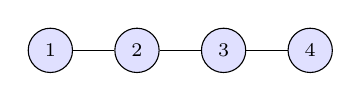
\begin{tikzpicture}
\foreach \i in {1,...,4}{\node[vtx,bluev] (a\i) at ({1.1*(\i-1)},0) {\i};}
\draw (a1)--(a2)--(a3)--(a4);
\end{tikzpicture}
\end{minipage}
\begin{minipage}{0.47\textwidth}\centering
UDG $H_1$
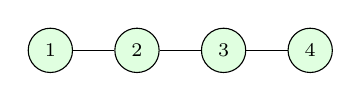
\begin{tikzpicture}
\foreach \i in {1,...,4}{\node[vtx,greenv] (b\i) at ({1.1*(\i-1)},0) {\i};}
\draw (b1)--(b2)--(b3)--(b4);
\end{tikzpicture}
\end{minipage}
\end{center}
\textit{Note.} No elimination. Vertices $1,2,3,4$ are preserved exactly.

\textbf{One valid colouring.}
\begin{center}
\begin{minipage}{0.47\textwidth}\centering
Colouring of $G_1$
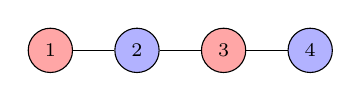
\begin{tikzpicture}
\node[vtx,c1] (a1) at (0,0) {1};
\node[vtx,c2] (a2) at (1.1,0) {2};
\node[vtx,c1] (a3) at (2.2,0) {3};
\node[vtx,c2] (a4) at (3.3,0) {4};
\draw (a1)--(a2)--(a3)--(a4);
\end{tikzpicture}
\end{minipage}
\begin{minipage}{0.47\textwidth}\centering
Colouring of $H_1$
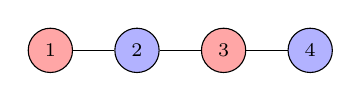
\begin{tikzpicture}
\node[vtx,c1] (b1) at (0,0) {1};
\node[vtx,c2] (b2) at (1.1,0) {2};
\node[vtx,c1] (b3) at (2.2,0) {3};
\node[vtx,c2] (b4) at (3.3,0) {4};
\draw (b1)--(b2)--(b3)--(b4);
\end{tikzpicture}
\end{minipage}
\end{center}

\section*{2. Property-preserving: $K_{3,3} \to C_6$}
\[
G_2=K_{3,3},\qquad H_2=C_6\in\UDG,\qquad \chi(G_2)=\chi(H_2)=2.
\]
\begin{center}
\begin{minipage}{0.47\textwidth}\centering
Original $G_2$
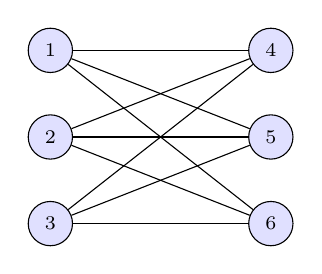
\begin{tikzpicture}
\foreach \i/\y in {1/1.1,2/0,3/-1.1}{\node[vtx,bluev] (L\i) at (0,\y) {\i};}
\foreach \i/\y in {4/1.1,5/0,6/-1.1}{\node[vtx,bluev] (R\i) at (2.8,\y) {\i};}
\foreach \i in {1,2,3}{\foreach \j in {4,5,6}{\draw (L\i)--(R\j);}}
\end{tikzpicture}
\end{minipage}
\begin{minipage}{0.47\textwidth}\centering
UDG $H_2$
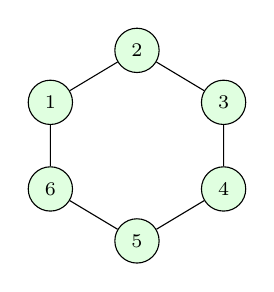
\begin{tikzpicture}
\foreach \i/\x/\y in {1/0/1,2/1/1.6,3/2/1,4/2/0,5/1/-0.6,6/0/0}{\node[vtx,greenv] (c\i) at (1.1*\x,1.1*\y) {\i};}
\draw (c1)--(c2)--(c3)--(c4)--(c5)--(c6)--(c1);
\end{tikzpicture}
\end{minipage}
\end{center}
\textit{Note.} No elimination in this illustrative example: both graphs have six vertices. However, the numbering does \emph{not} indicate an isomorphism; only the property $\chi=2$ is preserved.

\textbf{One valid colouring.}
\begin{center}
\begin{minipage}{0.47\textwidth}\centering
Colouring of $G_2$
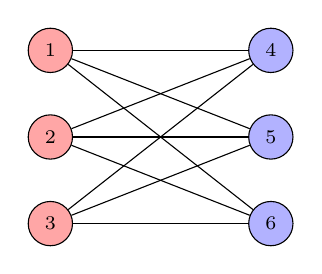
\begin{tikzpicture}
\foreach \i/\y in {1/1.1,2/0,3/-1.1}{\node[vtx,c1] (L\i) at (0,\y) {\i};}
\foreach \i/\y in {4/1.1,5/0,6/-1.1}{\node[vtx,c2] (R\i) at (2.8,\y) {\i};}
\foreach \i in {1,2,3}{\foreach \j in {4,5,6}{\draw (L\i)--(R\j);}}
\end{tikzpicture}
\end{minipage}
\begin{minipage}{0.47\textwidth}\centering
Colouring of $H_2$
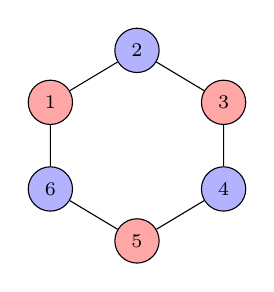
\begin{tikzpicture}
\node[vtx,c1] (c1) at (0,1.1) {1};
\node[vtx,c2] (c2) at (1.1,1.76) {2};
\node[vtx,c1] (c3) at (2.2,1.1) {3};
\node[vtx,c2] (c4) at (2.2,0) {4};
\node[vtx,c1] (c5) at (1.1,-0.66) {5};
\node[vtx,c2] (c6) at (0,0) {6};
\draw (c1)--(c2)--(c3)--(c4)--(c5)--(c6)--(c1);
\end{tikzpicture}
\end{minipage}
\end{center}

\section*{3. Property-preserving: Petersen graph $\to C_5$}
\[
\chi(G_3)=3,\qquad H_3=C_5\in\UDG,\qquad \chi(G_3)=\chi(H_3)=3.
\]
\begin{center}
\begin{minipage}{0.47\textwidth}\centering
Original $G_3$
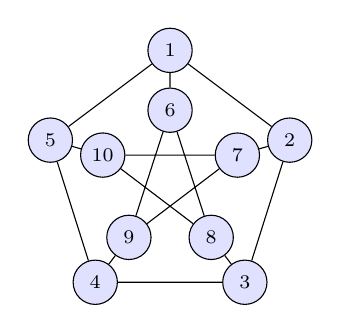
\begin{tikzpicture}[scale=0.95]
\foreach \i/\x/\y in {1/0/1.7,2/1.6/0.5,3/1.0/-1.4,4/-1.0/-1.4,5/-1.6/0.5}{\node[vtx,bluev] (o\i) at (\x,\y) {\i};}
\foreach \i/\x/\y in {6/0/0.9,7/0.9/0.3,8/0.55/-0.8,9/-0.55/-0.8,10/-0.9/0.3}{\node[vtx,bluev] (i\i) at (\x,\y) {\i};}
\draw (o1)--(o2)--(o3)--(o4)--(o5)--(o1);
\draw (i6)--(i8)--(i10)--(i7)--(i9)--(i6);
\draw (o1)--(i6) (o2)--(i7) (o3)--(i8) (o4)--(i9) (o5)--(i10);
\end{tikzpicture}
\end{minipage}
\begin{minipage}{0.47\textwidth}\centering
UDG $H_3$
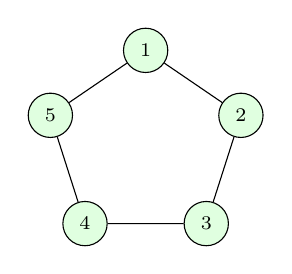
\begin{tikzpicture}
\foreach \i/\x/\y in {1/0/1.1,2/1.1/0.35,3/0.7/-0.9,4/-0.7/-0.9,5/-1.1/0.35}{\node[vtx,greenv] (p\i) at (1.1*\x,1.1*\y) {\i};}
\draw (p1)--(p2)--(p3)--(p4)--(p5)--(p1);
\end{tikzpicture}
\end{minipage}
\end{center}
\textit{Note.} Eliminated original vertices: $6,7,8,9,10$. The target keeps only a 5-vertex witness for $3$-colorability; exact structure is not preserved.

\textbf{One valid colouring.}
\begin{center}
\begin{minipage}{0.47\textwidth}\centering
Colouring of $G_3$
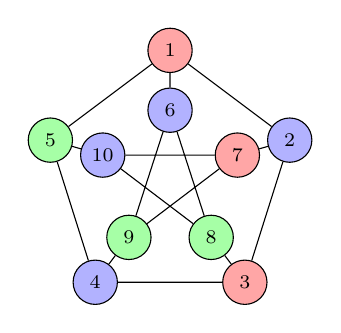
\begin{tikzpicture}[scale=0.95]
\node[vtx,c1] (o1) at (0,1.7) {1};
\node[vtx,c2] (o2) at (1.6,0.5) {2};
\node[vtx,c1] (o3) at (1.0,-1.4) {3};
\node[vtx,c2] (o4) at (-1.0,-1.4) {4};
\node[vtx,c3] (o5) at (-1.6,0.5) {5};
\node[vtx,c2] (i6) at (0,0.9) {6};
\node[vtx,c1] (i7) at (0.9,0.3) {7};
\node[vtx,c3] (i8) at (0.55,-0.8) {8};
\node[vtx,c3] (i9) at (-0.55,-0.8) {9};
\node[vtx,c2] (i10) at (-0.9,0.3) {10};
\draw (o1)--(o2)--(o3)--(o4)--(o5)--(o1);
\draw (i6)--(i8)--(i10)--(i7)--(i9)--(i6);
\draw (o1)--(i6) (o2)--(i7) (o3)--(i8) (o4)--(i9) (o5)--(i10);
\end{tikzpicture}
\end{minipage}
\begin{minipage}{0.47\textwidth}\centering
Colouring of $H_3$
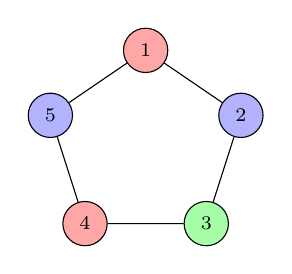
\begin{tikzpicture}
\node[vtx,c1] (p1) at (0,1.21) {1};
\node[vtx,c2] (p2) at (1.21,0.385) {2};
\node[vtx,c3] (p3) at (0.77,-0.99) {3};
\node[vtx,c1] (p4) at (-0.77,-0.99) {4};
\node[vtx,c2] (p5) at (-1.21,0.385) {5};
\draw (p1)--(p2)--(p3)--(p4)--(p5)--(p1);
\end{tikzpicture}
\end{minipage}
\end{center}

\section*{4. Property-preserving: $W_5 \to K_4$}
\[
\chi(G_4)=4,\qquad H_4=K_4\in\UDG,\qquad \chi(G_4)=\chi(H_4)=4.
\]
\begin{center}
\begin{minipage}{0.47\textwidth}\centering
Original $G_4$
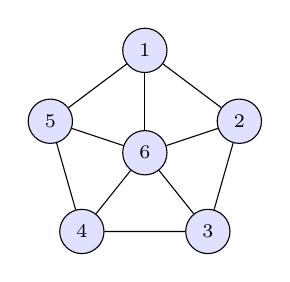
\begin{tikzpicture}
\foreach \i/\x/\y in {1/0/1.3,2/1.2/0.4,3/0.8/-1.0,4/-0.8/-1.0,5/-1.2/0.4}{\node[vtx,bluev] (w\i) at (\x,\y) {\i};}
\node[vtx,bluev] (h) at (0,0) {6};
\draw (w1)--(w2)--(w3)--(w4)--(w5)--(w1);
\foreach \i in {1,2,3,4,5}{\draw (h)--(w\i);} 
\end{tikzpicture}
\end{minipage}
\begin{minipage}{0.47\textwidth}\centering
UDG $H_4$
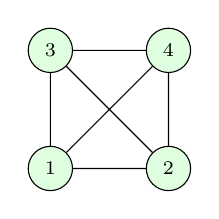
\begin{tikzpicture}
\node[vtx,greenv] (a) at (0,0) {1};
\node[vtx,greenv] (b) at (1.5,0) {2};
\node[vtx,greenv] (c) at (0,1.5) {3};
\node[vtx,greenv] (d) at (1.5,1.5) {4};
\draw (a)--(b)--(c)--(d)--(a)--(c) (b)--(d);
\end{tikzpicture}
\end{minipage}
\end{center}
\textit{Note.} Eliminated original vertices: $5,6$. The target keeps four mutually conflicting vertices as a witness for chromatic number $4$.

\textbf{One valid colouring.}
\begin{center}
\begin{minipage}{0.47\textwidth}\centering
Colouring of $G_4$
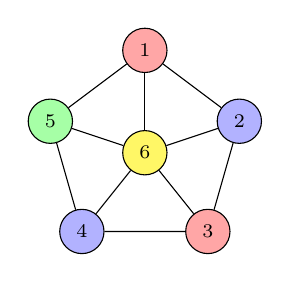
\begin{tikzpicture}
\node[vtx,c1] (w1) at (0,1.3) {1};
\node[vtx,c2] (w2) at (1.2,0.4) {2};
\node[vtx,c1] (w3) at (0.8,-1.0) {3};
\node[vtx,c2] (w4) at (-0.8,-1.0) {4};
\node[vtx,c3] (w5) at (-1.2,0.4) {5};
\node[vtx,c4] (h) at (0,0) {6};
\draw (w1)--(w2)--(w3)--(w4)--(w5)--(w1);
\foreach \i in {1,2,3,4,5}{\draw (h)--(w\i);} 
\end{tikzpicture}
\end{minipage}
\begin{minipage}{0.47\textwidth}\centering
Colouring of $H_4$
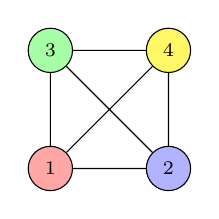
\begin{tikzpicture}
\node[vtx,c1] (a) at (0,0) {1};
\node[vtx,c2] (b) at (1.5,0) {2};
\node[vtx,c3] (c) at (0,1.5) {3};
\node[vtx,c4] (d) at (1.5,1.5) {4};
\draw (a)--(b)--(c)--(d)--(a)--(c) (b)--(d);
\end{tikzpicture}
\end{minipage}
\end{center}

\section*{5. Exact UDG: $P_5 \to P_5$}
\[
G_5=P_5,\qquad H_5\in\UDG,\qquad G_5\cong H_5.
\]
\begin{center}
\begin{minipage}{0.47\textwidth}\centering
Original $G_5$
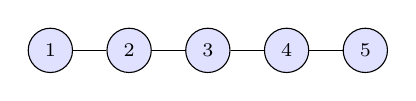
\begin{tikzpicture}
\foreach \i in {1,...,5}{\node[vtx,bluev] (v\i) at ({1.0*(\i-1)},0) {\i};}
\draw (v1)--(v2)--(v3)--(v4)--(v5);
\end{tikzpicture}
\end{minipage}
\begin{minipage}{0.47\textwidth}\centering
UDG $H_5$
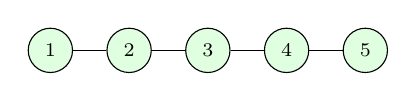
\begin{tikzpicture}
\foreach \i in {1,...,5}{\node[vtx,greenv] (u\i) at ({1.0*(\i-1)},0) {\i};}
\draw (u1)--(u2)--(u3)--(u4)--(u5);
\end{tikzpicture}
\end{minipage}
\end{center}
\textit{Note.} No elimination. Vertices $1$--$5$ are preserved exactly.

\textbf{One valid colouring.}
\begin{center}
\begin{minipage}{0.47\textwidth}\centering
Colouring of $G_5$
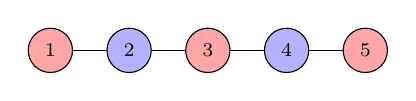
\begin{tikzpicture}
\node[vtx,c1] (v1) at (0,0) {1};
\node[vtx,c2] (v2) at (1,0) {2};
\node[vtx,c1] (v3) at (2,0) {3};
\node[vtx,c2] (v4) at (3,0) {4};
\node[vtx,c1] (v5) at (4,0) {5};
\draw (v1)--(v2)--(v3)--(v4)--(v5);
\end{tikzpicture}
\end{minipage}
\begin{minipage}{0.47\textwidth}\centering
Colouring of $H_5$
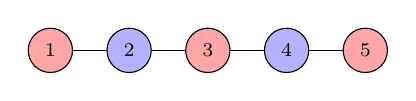
\begin{tikzpicture}
\node[vtx,c1] (u1) at (0,0) {1};
\node[vtx,c2] (u2) at (1,0) {2};
\node[vtx,c1] (u3) at (2,0) {3};
\node[vtx,c2] (u4) at (3,0) {4};
\node[vtx,c1] (u5) at (4,0) {5};
\draw (u1)--(u2)--(u3)--(u4)--(u5);
\end{tikzpicture}
\end{minipage}
\end{center}

\section*{6. Exact UDG: $C_4 \to C_4$}
\[
G_6=C_4,\qquad H_6\in\UDG,\qquad G_6\cong H_6.
\]
\begin{center}
\begin{minipage}{0.47\textwidth}\centering
Original $G_6$
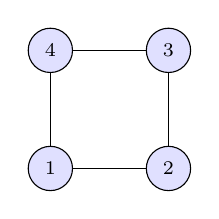
\begin{tikzpicture}
\node[vtx,bluev] (a) at (0,0) {1};
\node[vtx,bluev] (b) at (1.5,0) {2};
\node[vtx,bluev] (c) at (1.5,1.5) {3};
\node[vtx,bluev] (d) at (0,1.5) {4};
\draw (a)--(b)--(c)--(d)--(a);
\end{tikzpicture}
\end{minipage}
\begin{minipage}{0.47\textwidth}\centering
UDG $H_6$
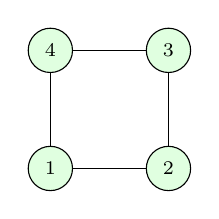
\begin{tikzpicture}
\node[vtx,greenv] (a) at (0,0) {1};
\node[vtx,greenv] (b) at (1.5,0) {2};
\node[vtx,greenv] (c) at (1.5,1.5) {3};
\node[vtx,greenv] (d) at (0,1.5) {4};
\draw (a)--(b)--(c)--(d)--(a);
\end{tikzpicture}
\end{minipage}
\end{center}
\textit{Note.} No elimination. Vertices $1,2,3,4$ are preserved exactly.

\textbf{One valid colouring.}
\begin{center}
\begin{minipage}{0.47\textwidth}\centering
Colouring of $G_6$
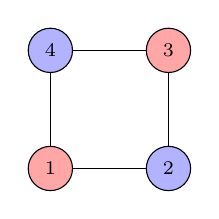
\begin{tikzpicture}
\node[vtx,c1] (a) at (0,0) {1};
\node[vtx,c2] (b) at (1.5,0) {2};
\node[vtx,c1] (c) at (1.5,1.5) {3};
\node[vtx,c2] (d) at (0,1.5) {4};
\draw (a)--(b)--(c)--(d)--(a);
\end{tikzpicture}
\end{minipage}
\begin{minipage}{0.47\textwidth}\centering
Colouring of $H_6$
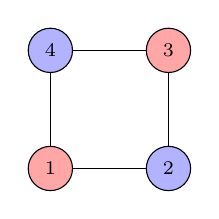
\begin{tikzpicture}
\node[vtx,c1] (a) at (0,0) {1};
\node[vtx,c2] (b) at (1.5,0) {2};
\node[vtx,c1] (c) at (1.5,1.5) {3};
\node[vtx,c2] (d) at (0,1.5) {4};
\draw (a)--(b)--(c)--(d)--(a);
\end{tikzpicture}
\end{minipage}
\end{center}

\section*{7. Exact UDG: $C_6 \to C_6$}
\[
G_7=C_6,\qquad H_7\in\UDG,\qquad G_7\cong H_7.
\]
\begin{center}
\begin{minipage}{0.47\textwidth}\centering
Original $G_7$
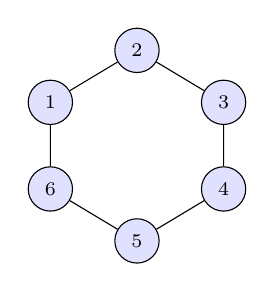
\begin{tikzpicture}
\foreach \i/\x/\y in {1/0/1,2/1/1.6,3/2/1,4/2/0,5/1/-0.6,6/0/0}{\node[vtx,bluev] (c\i) at (1.1*\x,1.1*\y) {\i};}
\draw (c1)--(c2)--(c3)--(c4)--(c5)--(c6)--(c1);
\end{tikzpicture}
\end{minipage}
\begin{minipage}{0.47\textwidth}\centering
UDG $H_7$
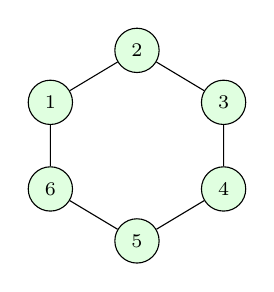
\begin{tikzpicture}
\foreach \i/\x/\y in {1/0/1,2/1/1.6,3/2/1,4/2/0,5/1/-0.6,6/0/0}{\node[vtx,greenv] (d\i) at (1.1*\x,1.1*\y) {\i};}
\draw (d1)--(d2)--(d3)--(d4)--(d5)--(d6)--(d1);
\end{tikzpicture}
\end{minipage}
\end{center}
\textit{Note.} No elimination. Vertices $1$--$6$ are preserved exactly.

\textbf{One valid colouring.}
\begin{center}
\begin{minipage}{0.47\textwidth}\centering
Colouring of $G_7$
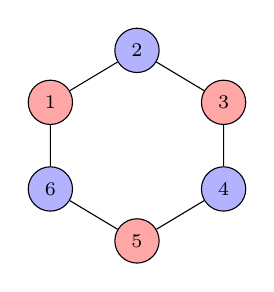
\begin{tikzpicture}
\node[vtx,c1] (c1) at (0,1.1) {1};
\node[vtx,c2] (c2) at (1.1,1.76) {2};
\node[vtx,c1] (c3) at (2.2,1.1) {3};
\node[vtx,c2] (c4) at (2.2,0) {4};
\node[vtx,c1] (c5) at (1.1,-0.66) {5};
\node[vtx,c2] (c6) at (0,0) {6};
\draw (c1)--(c2)--(c3)--(c4)--(c5)--(c6)--(c1);
\end{tikzpicture}
\end{minipage}
\begin{minipage}{0.47\textwidth}\centering
Colouring of $H_7$
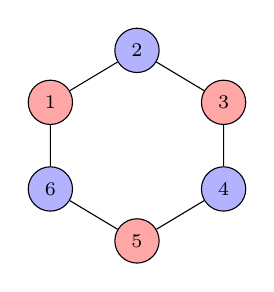
\begin{tikzpicture}
\node[vtx,c1] (d1) at (0,1.1) {1};
\node[vtx,c2] (d2) at (1.1,1.76) {2};
\node[vtx,c1] (d3) at (2.2,1.1) {3};
\node[vtx,c2] (d4) at (2.2,0) {4};
\node[vtx,c1] (d5) at (1.1,-0.66) {5};
\node[vtx,c2] (d6) at (0,0) {6};
\draw (d1)--(d2)--(d3)--(d4)--(d5)--(d6)--(d1);
\end{tikzpicture}
\end{minipage}
\end{center}

\section*{8. Exact UDG: $K_4 \to K_4$}
\[
G_8=K_4,\qquad H_8\in\UDG,\qquad G_8\cong H_8.
\]
\begin{center}
\begin{minipage}{0.47\textwidth}\centering
Original $G_8$
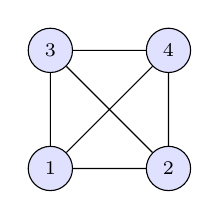
\begin{tikzpicture}
\node[vtx,bluev] (a) at (0,0) {1};
\node[vtx,bluev] (b) at (1.5,0) {2};
\node[vtx,bluev] (c) at (0,1.5) {3};
\node[vtx,bluev] (d) at (1.5,1.5) {4};
\draw (a)--(b)--(c)--(d)--(a)--(c) (b)--(d);
\end{tikzpicture}
\end{minipage}
\begin{minipage}{0.47\textwidth}\centering
UDG $H_8$
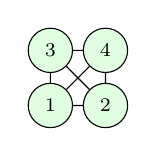
\begin{tikzpicture}
\node[vtx,greenv] (a) at (0.2,0.2) {1};
\node[vtx,greenv] (b) at (0.9,0.2) {2};
\node[vtx,greenv] (c) at (0.2,0.9) {3};
\node[vtx,greenv] (d) at (0.9,0.9) {4};
\draw (a)--(b)--(c)--(d)--(a)--(c) (b)--(d);
\end{tikzpicture}
\end{minipage}
\end{center}
\textit{Note.} No elimination. Vertices $1,2,3,4$ are preserved exactly.

\textbf{One valid colouring.}
\begin{center}
\begin{minipage}{0.47\textwidth}\centering
Colouring of $G_8$
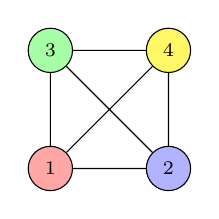
\begin{tikzpicture}
\node[vtx,c1] (a) at (0,0) {1};
\node[vtx,c2] (b) at (1.5,0) {2};
\node[vtx,c3] (c) at (0,1.5) {3};
\node[vtx,c4] (d) at (1.5,1.5) {4};
\draw (a)--(b)--(c)--(d)--(a)--(c) (b)--(d);
\end{tikzpicture}
\end{minipage}
\begin{minipage}{0.47\textwidth}\centering
Colouring of $H_8$
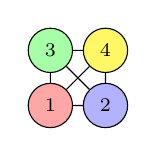
\begin{tikzpicture}
\node[vtx,c1] (a) at (0.2,0.2) {1};
\node[vtx,c2] (b) at (0.9,0.2) {2};
\node[vtx,c3] (c) at (0.2,0.9) {3};
\node[vtx,c4] (d) at (0.9,0.9) {4};
\draw (a)--(b)--(c)--(d)--(a)--(c) (b)--(d);
\end{tikzpicture}
\end{minipage}
\end{center}

\section*{9. Exact UDG: $K_5 \to K_5$}
\[
G_9=K_5,\qquad H_9\in\UDG,\qquad G_9\cong H_9.
\]
\begin{center}
\begin{minipage}{0.47\textwidth}\centering
Original $G_9$
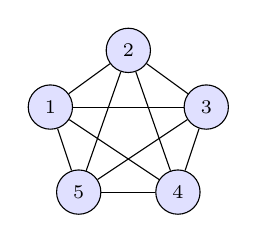
\begin{tikzpicture}[scale=0.9]
\foreach \i/\x/\y in {1/0/1.2,2/1.1/2,3/2.2/1.2,4/1.8/0,5/0.4/0}{\node[vtx,bluev] (v\i) at (\x,\y) {\i};}
\foreach \i in {1,2,3,4,5}{\foreach \j in {1,2,3,4,5}{\ifnum\i<\j\draw (v\i)--(v\j);\fi}}
\end{tikzpicture}
\end{minipage}
\begin{minipage}{0.47\textwidth}\centering
UDG $H_9$
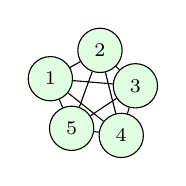
\begin{tikzpicture}[scale=0.9]
\foreach \i/\x/\y in {1/0.2/1.0,2/0.9/1.4,3/1.4/0.9,4/1.2/0.2,5/0.5/0.3}{\node[vtx,greenv] (u\i) at (\x,\y) {\i};}
\foreach \i in {1,2,3,4,5}{\foreach \j in {1,2,3,4,5}{\ifnum\i<\j\draw (u\i)--(u\j);\fi}}
\end{tikzpicture}
\end{minipage}
\end{center}
\textit{Note.} No elimination. Vertices $1$--$5$ are preserved exactly.

\textbf{One valid colouring.}
\begin{center}
\begin{minipage}{0.47\textwidth}\centering
Colouring of $G_9$
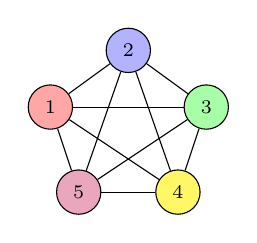
\begin{tikzpicture}[scale=0.9]
\node[vtx,c1] (v1) at (0,1.2) {1};
\node[vtx,c2] (v2) at (1.1,2) {2};
\node[vtx,c3] (v3) at (2.2,1.2) {3};
\node[vtx,c4] (v4) at (1.8,0) {4};
\node[vtx,c5] (v5) at (0.4,0) {5};
\foreach \i in {1,2,3,4,5}{\foreach \j in {1,2,3,4,5}{\ifnum\i<\j\draw (v\i)--(v\j);\fi}}
\end{tikzpicture}
\end{minipage}
\begin{minipage}{0.47\textwidth}\centering
Colouring of $H_9$
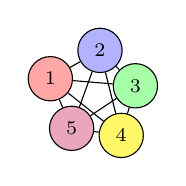
\begin{tikzpicture}[scale=0.9]
\node[vtx,c1] (u1) at (0.2,1.0) {1};
\node[vtx,c2] (u2) at (0.9,1.4) {2};
\node[vtx,c3] (u3) at (1.4,0.9) {3};
\node[vtx,c4] (u4) at (1.2,0.2) {4};
\node[vtx,c5] (u5) at (0.5,0.3) {5};
\foreach \i in {1,2,3,4,5}{\foreach \j in {1,2,3,4,5}{\ifnum\i<\j\draw (u\i)--(u\j);\fi}}
\end{tikzpicture}
\end{minipage}
\end{center}

\section*{10. Exact UDG: $K_{1,4} \to K_{1,4}$}
\[
G_{10}=K_{1,4},\qquad H_{10}\in\UDG,\qquad G_{10}\cong H_{10}.
\]
\begin{center}
\begin{minipage}{0.47\textwidth}\centering
Original $G_{10}$
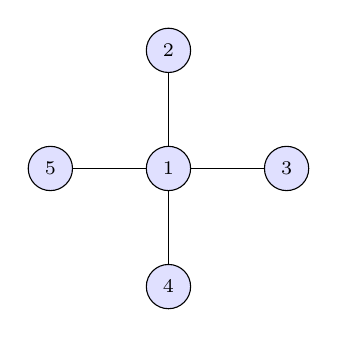
\begin{tikzpicture}
\node[vtx,bluev] (c) at (0,0) {1};
\node[vtx,bluev] (l1) at (0,1.5) {2};
\node[vtx,bluev] (l2) at (1.5,0) {3};
\node[vtx,bluev] (l3) at (0,-1.5) {4};
\node[vtx,bluev] (l4) at (-1.5,0) {5};
\draw (c)--(l1) (c)--(l2) (c)--(l3) (c)--(l4);
\end{tikzpicture}
\end{minipage}
\begin{minipage}{0.47\textwidth}\centering
UDG $H_{10}$
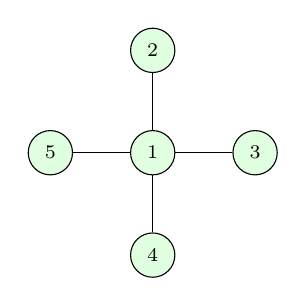
\begin{tikzpicture}
\node[vtx,greenv] (c) at (0,0) {1};
\node[vtx,greenv] (l1) at (0,1.3) {2};
\node[vtx,greenv] (l2) at (1.3,0) {3};
\node[vtx,greenv] (l3) at (0,-1.3) {4};
\node[vtx,greenv] (l4) at (-1.3,0) {5};
\draw (c)--(l1) (c)--(l2) (c)--(l3) (c)--(l4);
\end{tikzpicture}
\end{minipage}
\end{center}
\textit{Note.} No elimination. Vertices $1$--$5$ are preserved exactly.

\textbf{One valid colouring.}
\begin{center}
\begin{minipage}{0.47\textwidth}\centering
Colouring of $G_{10}$
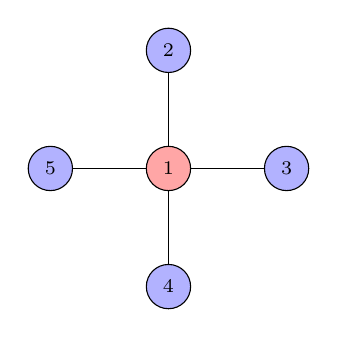
\begin{tikzpicture}
\node[vtx,c1] (c) at (0,0) {1};
\node[vtx,c2] (l1) at (0,1.5) {2};
\node[vtx,c2] (l2) at (1.5,0) {3};
\node[vtx,c2] (l3) at (0,-1.5) {4};
\node[vtx,c2] (l4) at (-1.5,0) {5};
\draw (c)--(l1) (c)--(l2) (c)--(l3) (c)--(l4);
\end{tikzpicture}
\end{minipage}
\begin{minipage}{0.47\textwidth}\centering
Colouring of $H_{10}$
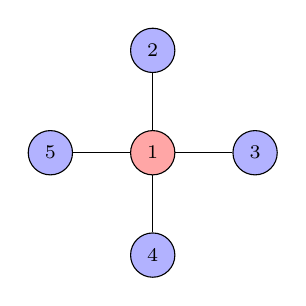
\begin{tikzpicture}
\node[vtx,c1] (c) at (0,0) {1};
\node[vtx,c2] (l1) at (0,1.3) {2};
\node[vtx,c2] (l2) at (1.3,0) {3};
\node[vtx,c2] (l3) at (0,-1.3) {4};
\node[vtx,c2] (l4) at (-1.3,0) {5};
\draw (c)--(l1) (c)--(l2) (c)--(l3) (c)--(l4);
\end{tikzpicture}
\end{minipage}
\end{center}

\section*{11. Property-preserving: $K_{2,3} \to C_4$}
\[
H_{11}=C_4\in\UDG,\qquad \chi(G_{11})=\chi(H_{11})=2.
\]
\begin{center}
\begin{minipage}{0.47\textwidth}\centering
Original $G_{11}=K_{2,3}$
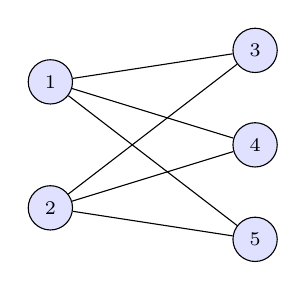
\begin{tikzpicture}
\node[vtx,bluev] (a1) at (0,0.8) {1};
\node[vtx,bluev] (a2) at (0,-0.8) {2};
\node[vtx,bluev] (b3) at (2.6,1.2) {3};
\node[vtx,bluev] (b4) at (2.6,0) {4};
\node[vtx,bluev] (b5) at (2.6,-1.2) {5};
\foreach \u in {a1,a2}{\foreach \v in {b3,b4,b5}{\draw (\u)--(\v);}}
\end{tikzpicture}
\end{minipage}
\begin{minipage}{0.47\textwidth}\centering
UDG $H_{11}$
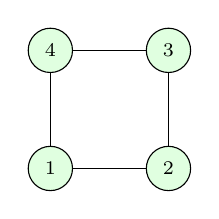
\begin{tikzpicture}
\node[vtx,greenv] (a) at (0,0) {1};
\node[vtx,greenv] (b) at (1.5,0) {2};
\node[vtx,greenv] (c) at (1.5,1.5) {3};
\node[vtx,greenv] (d) at (0,1.5) {4};
\draw (a)--(b)--(c)--(d)--(a);
\end{tikzpicture}
\end{minipage}
\end{center}
\textit{Note.} Eliminated original vertex: $5$. One vertex is dropped in the illustrative reduction because only bipartiteness / $2$-colorability is preserved.

\textbf{One valid colouring.}
\begin{center}
\begin{minipage}{0.47\textwidth}\centering
Colouring of $G_{11}$
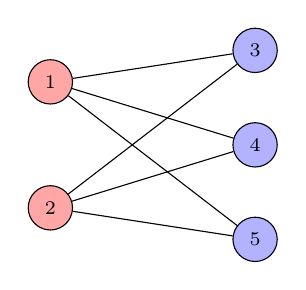
\begin{tikzpicture}
\node[vtx,c1] (a1) at (0,0.8) {1};
\node[vtx,c1] (a2) at (0,-0.8) {2};
\node[vtx,c2] (b3) at (2.6,1.2) {3};
\node[vtx,c2] (b4) at (2.6,0) {4};
\node[vtx,c2] (b5) at (2.6,-1.2) {5};
\foreach \u in {a1,a2}{\foreach \v in {b3,b4,b5}{\draw (\u)--(\v);}}
\end{tikzpicture}
\end{minipage}
\begin{minipage}{0.47\textwidth}\centering
Colouring of $H_{11}$
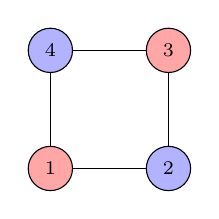
\begin{tikzpicture}
\node[vtx,c1] (a) at (0,0) {1};
\node[vtx,c2] (b) at (1.5,0) {2};
\node[vtx,c1] (c) at (1.5,1.5) {3};
\node[vtx,c2] (d) at (0,1.5) {4};
\draw (a)--(b)--(c)--(d)--(a);
\end{tikzpicture}
\end{minipage}
\end{center}

\section*{12. Property-preserving: house graph $\to C_5$}
\[
H_{12}=C_5\in\UDG,\qquad \chi(G_{12})=\chi(H_{12})=3.
\]
\begin{center}
\begin{minipage}{0.47\textwidth}\centering
Original house graph
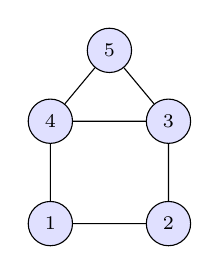
\begin{tikzpicture}
\node[vtx,bluev] (a) at (0,0) {1};
\node[vtx,bluev] (b) at (1.5,0) {2};
\node[vtx,bluev] (c) at (1.5,1.3) {3};
\node[vtx,bluev] (d) at (0,1.3) {4};
\node[vtx,bluev] (e) at (0.75,2.2) {5};
\draw (a)--(b)--(c)--(d)--(a) (d)--(e)--(c);
\end{tikzpicture}
\end{minipage}
\begin{minipage}{0.47\textwidth}\centering
UDG $H_{12}$
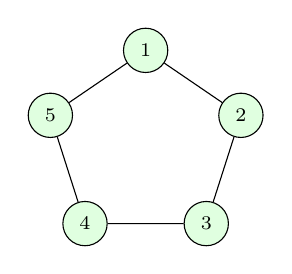
\begin{tikzpicture}
\foreach \i/\x/\y in {1/0/1.1,2/1.1/0.35,3/0.7/-0.9,4/-0.7/-0.9,5/-1.1/0.35}{\node[vtx,greenv] (p\i) at (1.1*\x,1.1*\y) {\i};}
\draw (p1)--(p2)--(p3)--(p4)--(p5)--(p1);
\end{tikzpicture}
\end{minipage}
\end{center}
\textit{Note.} No elimination. Both graphs have five vertices, but the numbering again does not indicate isomorphism; only the property $\chi=3$ is preserved.

\textbf{One valid colouring.}
\begin{center}
\begin{minipage}{0.47\textwidth}\centering
Colouring of $G_{12}$
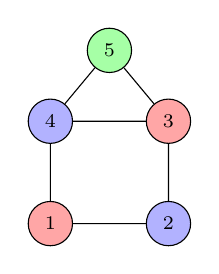
\begin{tikzpicture}
\node[vtx,c1] (a) at (0,0) {1};
\node[vtx,c2] (b) at (1.5,0) {2};
\node[vtx,c1] (c) at (1.5,1.3) {3};
\node[vtx,c2] (d) at (0,1.3) {4};
\node[vtx,c3] (e) at (0.75,2.2) {5};
\draw (a)--(b)--(c)--(d)--(a) (d)--(e)--(c);
\end{tikzpicture}
\end{minipage}
\begin{minipage}{0.47\textwidth}\centering
Colouring of $H_{12}$
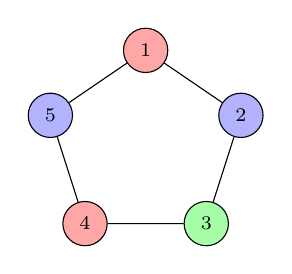
\begin{tikzpicture}
\node[vtx,c1] (p1) at (0,1.21) {1};
\node[vtx,c2] (p2) at (1.21,0.385) {2};
\node[vtx,c3] (p3) at (0.77,-0.99) {3};
\node[vtx,c1] (p4) at (-0.77,-0.99) {4};
\node[vtx,c2] (p5) at (-1.21,0.385) {5};
\draw (p1)--(p2)--(p3)--(p4)--(p5)--(p1);
\end{tikzpicture}
\end{minipage}
\end{center}

\section*{13. Property-preserving: bull graph $\to K_3$}
\[
H_{13}=K_3\in\UDG,\qquad \chi(G_{13})=\chi(H_{13})=3.
\]
\begin{center}
\begin{minipage}{0.47\textwidth}\centering
Original bull graph
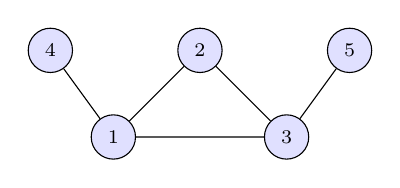
\begin{tikzpicture}
\node[vtx,bluev] (a) at (0,0) {1};
\node[vtx,bluev] (b) at (1.1,1.1) {2};
\node[vtx,bluev] (c) at (2.2,0) {3};
\node[vtx,bluev] (d) at (-0.8,1.1) {4};
\node[vtx,bluev] (e) at (3.0,1.1) {5};
\draw (a)--(b)--(c)--(a) (a)--(d) (c)--(e);
\end{tikzpicture}
\end{minipage}
\begin{minipage}{0.47\textwidth}\centering
UDG $H_{13}$
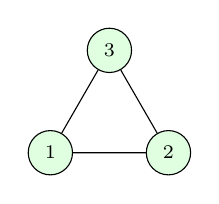
\begin{tikzpicture}
\node[vtx,greenv] (x) at (0,0) {1};
\node[vtx,greenv] (y) at (1.5,0) {2};
\node[vtx,greenv] (z) at (0.75,1.3) {3};
\draw (x)--(y)--(z)--(x);
\end{tikzpicture}
\end{minipage}
\end{center}
\textit{Note.} Eliminated original vertices: $4,5$. The two pendant vertices are removed because they do not change the fact that the graph has chromatic number $3$.

\textbf{One valid colouring.}
\begin{center}
\begin{minipage}{0.47\textwidth}\centering
Colouring of $G_{13}$
\begin{tikzpicture}
\node[vtx,c1] (a) at (0,0) {1};
\node[vtx,c2] (b) at (1.1,1.1) {2};
\node[vtx,c3] (c) at (2.2,0) {3};
\node[vtx,c2] (d) at (-0.8,1.1) {4};
\node[vtx,c2] (e) at (3.0,1.1) {5};
\draw (a)--(b)--(c)--(a) (a)--(d) (c)--(e);
\end{tikzpicture}
\end{minipage}
\begin{minipage}{0.47\textwidth}\centering
Colouring of $H_{13}$
\begin{tikzpicture}
\node[vtx,c1] (x) at (0,0) {1};
\node[vtx,c2] (y) at (1.5,0) {2};
\node[vtx,c3] (z) at (0.75,1.3) {3};
\draw (x)--(y)--(z)--(x);
\end{tikzpicture}
\end{minipage}
\end{center}

\section*{14. Property-preserving: $W_7 \to K_4$}
\[
H_{14}=K_4\in\UDG,\qquad \chi(G_{14})=\chi(H_{14})=4.
\]
\begin{center}
\begin{minipage}{0.47\textwidth}\centering
Original $G_{14}=W_7$
\begin{tikzpicture}[scale=0.9]
\foreach \i/\ang in {1/90,2/38,3/-14,4/-66,5/-118,6/-170,7/142}{\node[vtx,bluev] (r\i) at ({1.6*cos(\ang)},{1.6*sin(\ang)}) {\i};}
\node[vtx,bluev] (h) at (0,0) {8};
\draw (r1)--(r2)--(r3)--(r4)--(r5)--(r6)--(r7)--(r1);
\foreach \i in {1,2,3,4,5,6,7}{\draw (h)--(r\i);} 
\end{tikzpicture}
\end{minipage}
\begin{minipage}{0.47\textwidth}\centering
UDG $H_{14}$
\begin{tikzpicture}
\node[vtx,greenv] (a) at (0,0) {1};
\node[vtx,greenv] (b) at (1.5,0) {2};
\node[vtx,greenv] (c) at (0,1.5) {3};
\node[vtx,greenv] (d) at (1.5,1.5) {4};
\draw (a)--(b)--(c)--(d)--(a)--(c) (b)--(d);
\end{tikzpicture}
\end{minipage}
\end{center}
\textit{Note.} Eliminated original vertices: $5,6,7,8$. The target uses only four vertices as a witness for chromatic number $4$; the larger wheel structure is not retained.

\textbf{One valid colouring.}
\begin{center}
\begin{minipage}{0.47\textwidth}\centering
Colouring of $G_{14}$
\begin{tikzpicture}[scale=0.9]
\node[vtx,c1] (r1) at ({1.6*cos(90)},{1.6*sin(90)}) {1};
\node[vtx,c2] (r2) at ({1.6*cos(38)},{1.6*sin(38)}) {2};
\node[vtx,c1] (r3) at ({1.6*cos(-14)},{1.6*sin(-14)}) {3};
\node[vtx,c2] (r4) at ({1.6*cos(-66)},{1.6*sin(-66)}) {4};
\node[vtx,c1] (r5) at ({1.6*cos(-118)},{1.6*sin(-118)}) {5};
\node[vtx,c2] (r6) at ({1.6*cos(-170)},{1.6*sin(-170)}) {6};
\node[vtx,c3] (r7) at ({1.6*cos(142)},{1.6*sin(142)}) {7};
\node[vtx,c4] (h) at (0,0) {8};
\draw (r1)--(r2)--(r3)--(r4)--(r5)--(r6)--(r7)--(r1);
\foreach \i in {1,2,3,4,5,6,7}{\draw (h)--(r\i);} 
\end{tikzpicture}
\end{minipage}
\begin{minipage}{0.47\textwidth}\centering
Colouring of $H_{14}$
\begin{tikzpicture}
\node[vtx,c1] (a) at (0,0) {1};
\node[vtx,c2] (b) at (1.5,0) {2};
\node[vtx,c3] (c) at (0,1.5) {3};
\node[vtx,c4] (d) at (1.5,1.5) {4};
\draw (a)--(b)--(c)--(d)--(a)--(c) (b)--(d);
\end{tikzpicture}
\end{minipage}
\end{center}

\end{document}